\documentclass[prb,12pt]{revtex4-2}

\usepackage{amsmath, amssymb,physics,amsfonts,amsthm}
\usepackage{enumitem}
\usepackage{cancel}
\usepackage{booktabs}
\usepackage{tikz}
\usepackage{hyperref}
\usepackage{enumitem}
\usepackage{transparent}
\usepackage{float}
\usepackage{multirow}
\newtheorem{Theorem}{Theorem}
\newtheorem{Proposition}{Theorem}
\newtheorem{Lemma}[Theorem]{Lemma}
\newtheorem{Corollary}[Theorem]{Corollary}
\newtheorem{Example}[Theorem]{Example}
\newtheorem{Remark}[Theorem]{Remark}
\theoremstyle{definition}
\newtheorem{Problem}{Problem}
\theoremstyle{definition}
\newtheorem{Definition}[Theorem]{Definition}
\newenvironment{parts}{\begin{enumerate}[label=(\alph*)]}{\end{enumerate}}
%tikz
\usetikzlibrary{patterns}
% definitions of number sets
\newcommand{\N}{\mathbb{N}}
\newcommand{\R}{\mathbb{R}}
\newcommand{\Z}{\mathbb{Z}}
\newcommand{\Q}{\mathbb{Q}}
\newcommand{\C}{\mathbb{C}}
\begin{document}
\title{Vertiefung Analysis (Analysis 3)}
\author{Jun Wei Tan}
\email{jun-wei.tan@stud-mail.uni-wuerzburg.de}
\affiliation{Julius-Maximilians-Universit\"{a}t W\"{u}rzburg}
\date{\today}
\maketitle
\section{17/10/23}
Maß-und Integrationstheory
\subsection{Bücher}
\begin{enumerate}
	\item Escher Analysis III
	\item Forstes Analysis 3
	\item Elstratt Maß- und Integrationstheorie
\end{enumerate}

Kann man $A\subseteq \R^3$ Volumen zuweisen?

\paragraph{Inhaltsproblem} Man sollte eine Abbildung finden
\[
	m:\mathcal{P}\to [0,+\infty]
.\] 
Eigenschaften von $m$:
\begin{enumerate}
	\item \[
			m(A \cup B)=m(A)+m(B)\qquad \text{f\"{u}r}\qquad A\cap B = \varnothing
	.\] 
\item \[
m(A)=m(\beta(A))
,\] 
wobei $\beta: \R^n \to \R^n$ eine Bewegung ist.
\item \[
		m([0,1]^n)=1
,\]
\item Es hat f\"{u}r $n\ge 3$ keine l\"{o}sung.
\item Nicht trivial wegen des Banach-Tarski-Paradox
\end{enumerate}

Von (2) und (3) errichen wir die Folge

\begin{Theorem}
\[
m\left( \bigcup_{j=1}^\infty\right) = \sum_{j=1}^{\infty} m(A_j) 
,\]
f\"{u}r paarweise disjunkt, also
\[
A_i\cap A_j=\varnothing, i\neq j
.\] 
\end{Theorem}
\begin{proof}
	Es gibt \emph{keine} L\"{o}sung f\"{u}r alle $n$.
\end{proof}

\begin{Definition}
	Eine Teilmenge $\mathcal{A}\subseteq \mathcal{P}(X) \mathcal{A}\subseteq \mathcal{P}(X)$ heißt $\sigma-$ Algebra, falls es die folgende Eigenschaften hat:
	\begin{enumerate}
		\item $x\in \mathcal{A}$ 
		\item $A\in \mathcal{A}\implies A^c\in\mathcal{A}$
		\item $(A_j), A_j\in A\implies \bigcup_{j} A_j\in \mathcal{A}$
	\end{enumerate}
\end{Definition}

\begin{Theorem}
	Sei $A$ ein $\sigma$-Algebra \"{u}ber $X$. Dann
	\begin{enumerate}
		\item $\varnothing \in X$ 
		\item $A_1,A_2\in A\implies A_1\cap A_2\in X$ und $A_1 \\ A_2\in X$ 
		\item $(A_j) A_j\in X\implies \bigcap_{j}^\infty A_j\in X$
	\end{enumerate}
\end{Theorem}

\begin{proof}
	Beachten:
	\[
		A^c=\varnothing\in \mathcal{A}
	.\] 
	\[
	A_1\cap A_2=\qty(A_1^c\cup A_2^c)^c
	.\] 
	\[
	A_1 \\ A_2=A_1\cap A_2^c
	.\] 
	\[
	\bigcap_{j=1}^\infty A_j=\left( \bigcup_{j=1}^\infty A_j^c \right)^c
	.\] 
\end{proof}

\begin{Example}
	Sei $X=\left\{ 1,2,3 \right\} $. Dann ist
	\[
		\mathcal{A}=\left\{ \varnothing, X, \left\{ 1,2 \right\} , \left\{ 3 \right\}  \right\} \] 
		ein $\sigma-$ Algebra.
\end{Example}

\begin{Theorem}
	Sei $\mathcal{A}$ und $\mathcal{B}$ $\sigma$-Algebren \"{u}ber $X$ und $Y$. Dann sind
	\begin{gather*}
		f^{-1}(\mathcal{B})=\left\{ f^{-1}(B), B\in\mathcal{B} \right\} \\
		f_*(\mathcal{A})=\left\{ B\subseteq Y: f^{-1}(B)\in \mathcal{A} \right\} 
	\end{gather*}
	auch $\sigma$-Algebren
\end{Theorem}

\begin{proof}
	Wir beweisen es nur f\"{u}r $f_*$.
	\begin{enumerate}
		\item $Y\in f_*(\mathcal{A})$, weil $f^{-1}(Y)=X\in \mathcal{A}$ 
		\item Sei $B\in f_x(\mathcal{A})$. Dann gilt
			\[
				f^{-1}\left( B^c \right) =\left( f^{-1}(B) \right)^c\in \mathcal{A}
			.\] 
		\item Sei $(B_j), B_j\in f_*(\mathcal{A}\forall j$. Dann ist
			\[
				f^{-1}\left( \bigcup_{j=1} ^\infty B_j \right) =\bigcup_{j=1} ^\infty f^{-1}(B_j)\in \mathcal{A}
			.\] 
	\end{enumerate}
\end{proof}

\begin{Lemma}
	Sei $I$ nichtleer, und $\mathcal{A}_i$ $\sigma$-Algebren f\"{u}r jeder $i\in I$. Dann ist
	\[
		\bigcap_{i\in I} \mathcal{A}_i
	\] ein $\sigma$-Algebra
\end{Lemma}

\begin{Definition}
	Sei $X\subseteq \mathcal{P}(X)$. Dann wird es definiert
	\[
		A_\sigma(S)=\bigcap \left\{ \mathcal{A}: \mathcal{A} \text{ ist ein $\sigma$-Algebra mit } S\subseteq \mathcal{A} \right\}  
	.\] 
\end{Definition}

\begin{Corollary}
	Ist $\mathcal{A}$ $\sigma$-Algebra mit $S\subseteq \mathcal{A}$, dann 
	\[
		\mathcal{A}_\sigma(S)\subseteq\mathcal{A}
	.\] 
\end{Corollary}

\begin{Theorem}
	Die Abbildung $S\to A_\sigma(S)$ hat folgende Eigenschaften:
	\begin{enumerate}
		\item $S\subseteq \mathcal{A}_\sigma(S)$ 
		\item $S\subseteq T \subseteq \mathcal{P}(X)\implies \mathcal{A}_\sigma(S)\subseteq \mathcal{A}_\sigma(T)$ 
		\item $A_\sigma(A_\sigma(S))=A_\sigma(S)$
	\end{enumerate}
\end{Theorem}

\begin{Example}
	Sei $S=\left\{ \left\{ x \right\} , x\in X \right\} $. Dann ist
	\[
		\mathcal{A}_\sigma(S)=\left\{ A\subset X, A\text{ oder }A^c\text{ abz\"{a}hlbar (countable)} \right\} 
	.\] 
\end{Example}

\begin{proof}
	\begin{enumerate}
		\item $x\in A$ weil $A^c=\varnothing$ ist abz\"{a}hlbar
		\item Es ist klar, dass $A\in \mathcal{A}\implies A^c\in\mathcal{C}$.
		\item Sei $(A_j), A_j\in \mathcal{A}$. Dann, entweder
			\begin{enumerate}
				\item alle $A_j$ abz\"{a}hlbar sind und daher
					\[
					\bigcup_{j=1} ^\infty A_j
					.\] 
					abz\"{a}hlbar ist, oder mindestens eine $A_j^c$ abz\"{a}hlbar ist, wobei
					\[
					\qty(\bigcup_{j=1} ^\infty A_j)^c=\bigcap_{j=1}^\infty A_j^c\] 
					abz\"{a}hlbar ist.
			\end{enumerate}
		\item Zu zeigen:
			\[
				\mathcal{A}\subseteq \mathcal{A}_\sigma(S)
			.\] 
			Sei $A\in \mathcal{A}$. Angenommen A ist abz\"{a}hlbar. Dann 
			\[
			A=\bigcup_{j=1} \infty \left\{ a_j \right\} \in A_\sigma(S)
			.\] 
	\end{enumerate}
\end{proof}
\begin{Definition}
	Sei $(X, d)$ metrischer Raum. Dann ist $\mathcal{\tau}$ die Menge alle offene Menge. Wir definiert
	\[
		\mathcal{B}(X):=A_\sigma(\mathcal{\tau})
	\]
	und nennt das als das Borel-$\sigma$-Algebra.
\end{Definition}
\paragraph{Frage} Warum muss das ein metrischer Raum sein?

\begin{Theorem}
	Sei $(X,d)$ ein metrischer Raum. Sei $\mathcal{C}$ die Menge der abgeschlossenen Mengen und $\mathcal{K}$ die menge der kompakten Mengen. Dann ist 
	\begin{gather*}
		\mathcal{B}(X)=\mathcal{A}_\sigma(\mathcal{C})
	\end{gather*}

	Es existiert auch $K_j$ kompakt, wof\"{u}r gilt
	\[
		\mathcal{B}(X)=\mathcal{A}_\sigma(\mathcal{K})
	\] 
	wobei $X=\bigcup_{j=1} ^\infty K_j$
\end{Theorem}

\begin{proof}
\begin{enumerate}
	\item $\mathcal{A}$ offen $\iff$ $A^c$ abgeschlossen
	\item Kompakte Menge sind abgeschlossen $\implies A_\sigma(\mathcal{K})\subseteq A_\sigma(\mathcal{C})$.

		Sei $\mathcal{C}$ abgeschlossen. Dann gilt 
		\[
			C=C\cap X=C\cap \left( \bigcup_{j=1} ^\infty K_j \right) =\bigcup_{j=1} ^\infty\left( \underbrace{C\cap K_j}_\text{kompakt} \right) \in A_\sigma(K)
		.\] 
\end{enumerate}

\begin{Definition}
	Sei $a,b\in \R^n$. Dann definieren wir
	\[
	a\le b\\iff a_i \le b_i \forall i\in \left\{ 1,2,\dots, n \right\} 
	.\] 
\end{Definition}
\end{proof}

\section{18/10/23}
\begin{Theorem}
	 Jede offene Menge des $\R^n$ ist eine disjunkte abzählbare Vereinigung von halboffenen Würfeln mit rationalen Eckpunkten.
\end{Theorem}

\begin{proof}
	F\"{u}r $k\in \N$ definiere
	\[
		M_k :=\left\{ \left( \prod_{i=1}^n \left[\frac{x_i}{2^k}, \frac{x_i+1}{2^k}\right) \right),x\in \Z^n \right\} 
	.\] 
	\begin{center}
	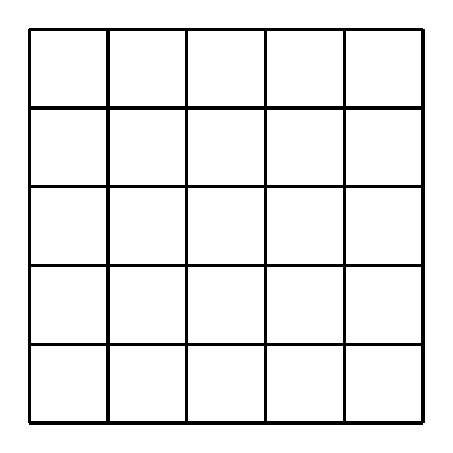
\begin{tikzpicture}
		\draw[very thick] (0,0) grid (5,5);
	\end{tikzpicture}
	\vspace{1cm}

	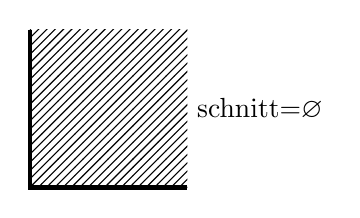
\begin{tikzpicture}[scale=2]
	\fill[pattern = north east lines] (0,0) rectangle (1,1);
	\draw[ultra thick] (0,1) -- (0,0) -- (1,0);
	\draw (1,0.5) node[anchor=west] {schnitt=$\varnothing$};
\end{tikzpicture}
\end{center}

Dann


\def\svgwidth{0.8\textwidth}
\input{diagram1.pdf_tex}
\end{proof}
\begin{Remark}
	(Produkt $\sigma$-Algebra) Sei $(X_1,\mathcal{A}_1)$ und $(X_2,\mathcal{A}_2)$ $\sigma$-Algebren. Wir bildet man ein $\sigma$-Algebra auf $X_1\times X_2$?

	Leider ist
	\[
		\left\{ A_1\times A_2,A_1\in\mathcal{A}_1, A_2\in \mathcal{A}_2 \right\} 
	.\] 
	kein $\sigma$-Algebra.

	\begin{center}
		\begin{tikzpicture}
			\draw[thick, ->] (0,0) -- (4,0);
			\draw[thick, ->] (0,0) -- (0,4);
			\draw[thick] (1,1) rectangle ++(1,1);
			\draw[thick] (1.5,1.5) rectangle ++(1,1);
		\end{tikzpicture}
	\end{center}
	Leider ist die Vereinigung kein Produkt-Menge
\end{Remark}
\section{24/10/23}
\begin{Definition}
	Sei $\mathcal{A}$ eine $\sigma$-Algebra \"{u}ber X, und $\mu:\mathcal{A}\to [0,\infty]$ Mengefunktion. Wenn $\mu$ $\sigma$-Additiv ist, heißt $\mu$ Maß. 

	Ist $\mu(X)=1$, dann heißt $\mu$ Wahrscheinlichkeitsmaß.
\end{Definition}
\begin{Example}
	Sei
	\[
	\varphi(A)=\begin{cases}
		1 & A \neq \varphi\\
		0 & A = \varphi
	\end{cases}
	.\] 
	Dann ist $\varphi$ endlich und $\sigma$-subadditiv. Aber weil es nicht $\sigma$-Additiv ist, ist es keinen Maß. 
\end{Example}
\begin{Definition}
	Sei $(X, \mathcal{A})$ eine $\sigma$-Algebra \"{u}ber $X$ und $a\in X$. Dann ist
	\[
	\varphi(A)=\begin{cases}
		1 & a \in A\\
		0 & a \not\in A
	\end{cases}
	.\] 
	ein Maß (Dirac-Maß)
\end{Definition}
\begin{Example}
	Sei $\varphi(A)=\text{ anzahl der Elemente von }A$. Dann ist $\varphi$ ein Maß. 
\end{Example}

\begin{Theorem}
	\begin{enumerate}
		\item $\mu(A \cap B)+\mu(A \cup B)=\mu(A)+\mu(B)$
		\item Falls $A\subseteq B$, dann ist $\mu(B\backslash A)=\mu(B)-\mu(A)$.
		\item Falls $A\subseteq B$, dann $\mu(A)\le \mu(B)$
		\item Falls $A_1\subseteq A_2\subseteq A_3\dots$,. dann $\lim_{k \to \infty} \mu(A_k)=\mu\left( \bigcup_{j=1} ^\infty A_j \right) $.
		\item Falls $A_1\supseteq A_2\supseteq A_3\dots$ und $\mu(A_1)<\infty$, dann ist $\lim_{k \to \infty} \mu(A_k)=\mu\left( \bigcap_{j=1} ^\infty A_j \right) $
	\end{enumerate}
\end{Theorem}

\begin{proof}
	\begin{enumerate}
		\item 
			\begin{align*}
				A \cup B=&A\cup(B\backslash A)\\
				B =& (B\backslash A)\cup (A \cap B)\\
				\mu(B\backslash A)=&\mu(A\cup B)-\mu(A)=\mu(B)-\mu(A \cap B)\\
				\mu(A\cup B)+\mu(A\cap B)=& \mu(A)+\mu(B)
			\end{align*}
		\item $B=A\cup (B\backslash A)$, und daher $\mu(B)=\mu(A)+\mu(B\backslash A)$.
		\item $\mu(B)=\mu(A)+\mu(B\backslash A)\ge \mu(A)$.
	\end{enumerate}
	\end{proof}
	\begin{Definition}
		Eine Menge $M\in \mathcal{A}$ heißt Nullmenge, Falls $\mu(M) =0$. Der Maßraum heißt vollständig, wenn gilt: $M \subseteq N, N$ Nullmenge impliziert $M\in \mathcal{A}$ (alle Teilmenge von Nullmengen sind messbar)
	\end{Definition}
	\begin{Corollary}
		Abz\"{a}hlbare Vereinigung von Nullmengen ist Nullmenge.
	\end{Corollary}
\begin{Definition}
	Eine Abbildung $\mu^*:[0,+\infty]$ heißt äußeres Maß, falls gilt:
	\begin{enumerate}
		\item $\mu^*(\varnothing)=0$ 
		\item $\mu*$ ist monoton, d.h $A\subseteq B\implies \mu^*(A)\le \mu^*(B)$ 
		\item $\mu^*$ ist $\sigma$-subadditiv
	\end{enumerate}
\end{Definition}
\section{12/12/23}
Unterschied zwischen alle 4 Variante des Satzes von Fubinis:

Satz 2.84: Positiv, messbar, integrierbarkeit nicht angenommen

Satz 2.85: Positivheit nicht angenommen, aber messbarkeit und integrierbarkeit angenommen,
\end{document}
